\documentclass[runningheads]{llncs}

\usepackage{graphicx}
\usepackage{amsmath}
\usepackage{amssymb}
\usepackage{booktabs}
\usepackage{multirow}
\usepackage{array}
\usepackage{url}
\usepackage{algorithm}
\usepackage{algorithmic}
\usepackage{subcaption}
\usepackage{mdframed}
\usepackage{hyperref}
\usepackage{tikz}
\usetikzlibrary{positioning}
\usepackage{pgfplots}
\usepackage{float}
\pgfplotsset{compat=1.18}

\bibliographystyle{splncs04}

\begin{document}

\title{Emotional Models: Text Mood Classification}
\author{
    Miguel Cabral Pinto\inst{1} \and Tiago Silva\inst{2} \\
    \email{\inst{1}mcp@student.uc.pt, \inst{2}tds@student.uc.pt}
}
\authorrunning{M. Cabral Pinto \and T. Silva}
\institute{
    Department of Informatics Engineering \\ University of Coimbra \\ Coimbra, Portugal\\
}

\maketitle

\begin{abstract}
    This project explores the classification of emotional states in text using supervised and zero-shot learning approaches. 
    We implement and compare artificial neural networks (ANNs) and transformer-based models to categorize text into six emotion classes. 
    The methodology includes training ANNs for various epochs and evaluating their performance using confusion matrices and accuracy metrics. 
    Additionally, we assess large pre-trained BERT models in a zero-shot setting, in order to draw comparisons between the two approaches. 
    Experimental results demonstrate the effectiveness of both supervised and zero-shot models, with comparative analysis highlighting their strengths and limitations for these sorts of tasks.

    \keywords{Emotion Classification \and Supervised Learning \and Zero-shot Learning \and BERT \and Artificial Neural Networks}
\end{abstract}

\section{Methodology}

\subsection{Dataset}

For the purpose of classifying emotional states in text, we utilize the dataset requested in the project statement (HuggingFace's \texttt{dair-ai/emotion}\footnote{\url{https://huggingface.co/datasets/dair-ai/emotion}}), consisting of labeled examples across six emotion categories: sadness, joy, love, anger, fear, and surprise.
The characteristics of its split version, which will be used in this project, are as follows:

\begin{itemize}
    \item \textbf{Source:} Social media (Twitter) messages
    \item \textbf{Language:} English
    \item \textbf{Text Length:} 7 \textrightarrow~300 characters
    \item \textbf{Classes:} 6 (sadness, joy, love, anger, fear, surprise)
    \item \textbf{Training Set:} 16000 labeled examples
    \item \textbf{Validation Set:} 2000 labeled examples
    \item \textbf{Test Set:} 2000 labeled examples
    \item \textbf{Total:} 20000 labeled examples
\end{itemize}

\begin{figure}[htbp]
    \centering
    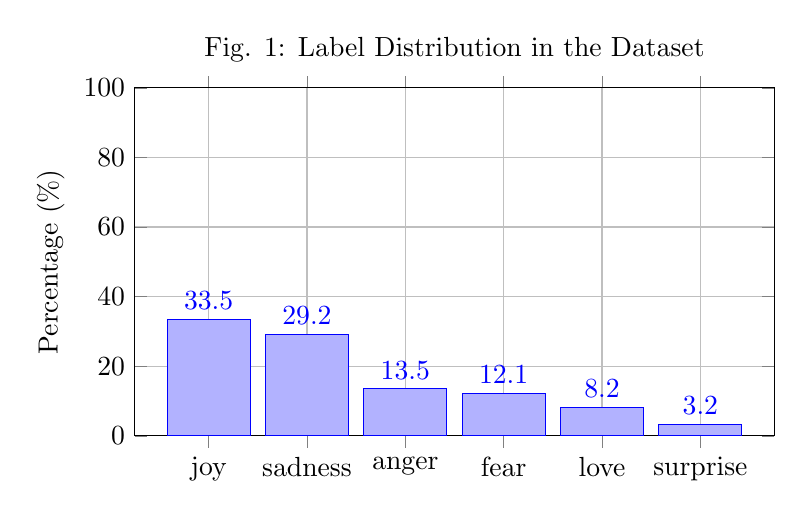
\begin{tikzpicture}
        \begin{axis}[
            ybar,
            bar width=30pt,
            width=0.8\textwidth,
            height=6cm,
            ymin=0,
            ymax=100,
            xtick=data,
            xticklabels={joy, sadness, anger, fear, love, surprise},
            ylabel={Percentage (\%)},
            title={Fig. 1: Label Distribution in the Dataset},
            nodes near coords,
            nodes near coords align={vertical},
            enlarge x limits=0.15,
            grid=major,
        ]
        \addplot coordinates {(0,33.5) (1,29.2) (2,13.5) (3,12.1) (4,8.2) (5,3.2)};
        \end{axis}
    \end{tikzpicture}
    \label{fig:label_distribution}
\end{figure}
\vspace{-10pt}

\noindent Upon initially looking at the data, a challenge immediately became apparent: class imbalance. 
Rarer emotions are heavily misrepresented (only 3.2\% of examples have a ``surprise'' label), while simpler, more common emotions which may overlap with others dominate the dataset (the ``joy'' and ``sadness'' classes hold a joint 62.7\% of the examples).
This is an issue because the model can specialize in a subset of the classes and be biased towards them.
In this case, completely ignoring ``surprise'' but getting every other example right would give the model a misleadingly high accuracy of approximately 96.8\%.
This is one of the reasons why accuracy alone is not a sufficient metric for evaluating model performance in this context, and why confusion matrices and other metrics computed from them (particularly those that measure per-class performance) are very important.
This dataset imbalance has other implications as well, specially when comparing two diferent paradigms (supervised learning and zero-shot classification), as each may be affected differently by the lack of data for certain classes.
On the one hand we have the ANNs which are directly harmed by the lack of class representation because they learn from the empirical distribution of the data, affecting the decision boundaries they create. 
On the other hand we have the zero-shot models which dont learn from the data, contrastingly they may be less affected by class imbalance, but their performance may still vary across classes due to the inherent biases in the pre-trained models they rely on.

\noindent Another problem that stands out when analyzing the data is the reliability of its labels.
Several of the data points show text-label pairs with a mismatch that is obvious to a human eye, with the most common pattern being lack of context undestanding.
For example, texts like \textit{i no longer feel happy to score well} and \textit{i never feel that popular} were both labeled as ``joy'' due to their use of \textit{happy} and \textit{popular}, words that usually convey positive emotions, even though in these cases their negation is used, causing the overall sentiment to be reversed.
Inconsistencies such as these mean that there is a cap to the performance of any model on this dataset, unless it overfits to the noise in the labels (even then, it is not guaranteed that the training and testing sets will have the same types of mismatches).
This is shown by Kermani et al.\cite{kermani2025systematicevaluationllmstrategies} as their attempt at fine-tuning an extensive model (LLaMA-38B) for this task achieves the best performance out of the tried approaches (including zero-shot classification, which is explored in this project) at 91\%.

\noindent In order to understand the dataset better, it is important to consider how it was populated.
Though no information is provided in the HuggingFace website on this aspect, the GitHub repository containing the data\footnote{\url{https://github.com/dair-ai/emotion_dataset}} links to a paper by the authors that details the creation process \cite{saravia-etal-2018-carer} (though the repository and paper do not refer to the same dataset, they are populated in the same manner).
The proposed model, CARER, consists of a semi-supervised, graph-based algorithm designed to create contextualized emotion representations that relies on \textit{enriched patterns}, which identify similar text structures across examples to help with classification.
However, our manual analysis suggests that while the CARER method aims to account for context, its application in creating this specific dataset may not have fully overcome the challenge of syntactic nuance, leaving a pattern of keyword-emotion association in some entries.

\subsection{Experimental Pipeline}
The main goal of this project is to explore and compare supervised and zero-shot learning approaches for emotion classification using a modular and reproducible experimental setup.
The pipeline to fulfill this goal is illustrated in Figure~\ref{fig:pipeline}, showcasing the two main approaches: supervised learning using artificial neural networks (ANNs) and zero-shot classification with pre-trained transformer models.

\begin{figure}[htbp]
    \centering
    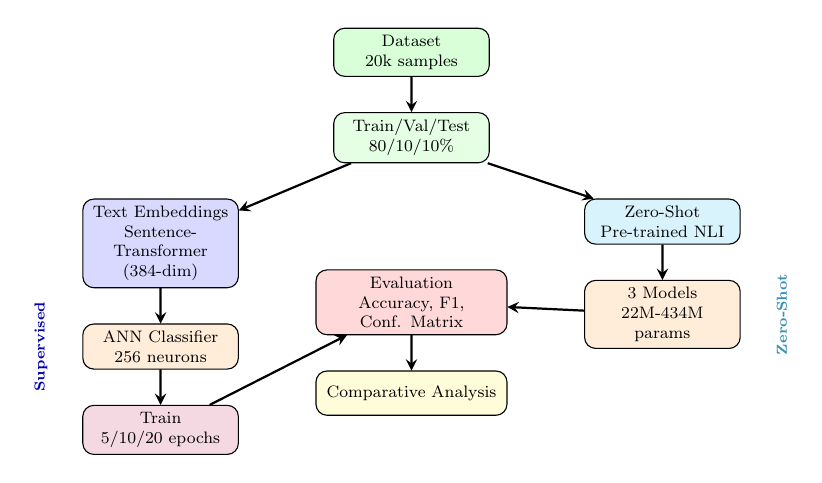
\begin{tikzpicture}[
        scale=0.75,
        transform shape,
        node distance=0.9cm and 1.2cm,
        box/.style={rectangle, draw, fill=blue!15, text width=2.4cm, align=center, rounded corners, minimum height=0.75cm, font=\footnotesize},
        arrow/.style={->, >=stealth, thick}
    ]
    
    % Top: Dataset
    \node[box, fill=green!15] (data) {Dataset\\20k samples};
    
    % Split
    \node[box, fill=green!10, below=0.6cm of data] (split) {Train/Val/Test\\80/10/10\%};
    
    % Supervised branch (left)
    \node[box, fill=blue!15, below left=0.6cm and 1.6cm of split] (embed) {Text Embeddings SentenceTransformer\\(384-dim)};
    \node[box, fill=orange!15, below=0.6cm of embed] (ann) {ANN Classifier\\256 neurons};
    \node[box, fill=purple!15, below=0.6cm of ann] (train) {Train\\5/10/20 epochs};
    
    % Zero-shot branch (right)
    \node[box, fill=cyan!15, below right=0.6cm and 1.6cm of split] (zs) {Zero-Shot\\Pre-trained NLI};
    \node[box, fill=orange!15, below=0.6cm of zs] (models) {3 Models\\22M-434M params};
    
    % Evaluation (bottom center)
    \node[box, fill=red!15, text width=3cm, below=1.8cm of split] (eval) {Evaluation\\Accuracy, F1, Conf. Matrix};
    
    % Comparison (final)
    \node[box, fill=yellow!15, text width=3cm, below=0.6cm of eval] (comp) {Comparative Analysis};
    
    % Arrows
    \draw[arrow] (data) -- (split);
    \draw[arrow] (split) -- (embed);
    \draw[arrow] (embed) -- (ann);
    \draw[arrow] (ann) -- (train);
    \draw[arrow] (train) -- (eval);
    \draw[arrow] (split) -- (zs);
    \draw[arrow] (zs) -- (models);
    \draw[arrow] (models) -- (eval);
    \draw[arrow] (eval) -- (comp);
    
    \node[text=blue!70!black, font=\scriptsize\bfseries, rotate=90] at ([xshift=-0.7cm]ann.west) {Supervised};
    \node[text=cyan!70!black, font=\scriptsize\bfseries, rotate=90] at ([xshift=0.7cm]models.east) {Zero-Shot};
        
    \end{tikzpicture}
    \caption{Experimental pipeline overview: supervised learning (left) trains an ANN on embeddings, while zero-shot (right) uses pre-trained models directly.}
    \label{fig:pipeline}
\end{figure}

\subsection{Implementation}
The entire source code for this project is implemented in Python and organized into modular scripts to facilitate experimentation.

\noindent The supervised learning pipeline is defined in \texttt{supervised.py}, which is an adaptation of the code initially provided with this assignment, where artificial neural networks (ANNs) are constructed and trained using the dataset. 
The script relies on PyTorch for model definition, training, and evaluation. 
Training progress and results, including confusion matrices and accuracy metrics, are logged for analysis. 
The main orchestration of experiments, including data loading, model selection, and evaluation, is handled in \texttt{main.py}.

\noindent For zero-shot classification, \texttt{zero\_shot.py} utilizes transformer models from the HuggingFace library, such as BERT.
It differs from the previous approach by performing data point classification without explicit training on the dataset labels, instead infering emotions directly from text using pre-trained language representations.
The selected models for zero-shot classification aim to cover a range of sizes and capabilities, from large models like BART-large-mnli to more compact ones like DeBERTa-v3-xsmall-zeroshot, allowing for a comparative analysis of performance versus computational efficiency.

\noindent The following table summarizes the models evaluated in both supervised and zero-shot settings:

\vspace{-15pt}
\begin{table}[htbp]
    \centering
    \caption{Model Specifications and Configurations}
    \label{tab:model_specs}
    \begin{tabular}{lcc}
        \toprule
        \textbf{Model} & \textbf{Parameters} & \textbf{Training Objective} \\
        \midrule
        \multicolumn{3}{c}{\textit{Supervised Approach}} \\
        \midrule
        ANNClassifier (5 epochs) & 98,566 & Cross-Entropy Loss \\
        ANNClassifier (10 epochs) & 98,566 & Cross-Entropy Loss \\
        ANNClassifier (20 epochs) & 98,566 & Cross-Entropy Loss \\
        \midrule
        \multicolumn{3}{c}{\textit{Zero-Shot Approach}} \\
        \midrule
        BART-large-mnli & 406M & NLI (MNLI) \\
        DeBERTa-v3-large-zeroshot & 434M & NLI + Zero-shot \\
        DeBERTa-v3-xsmall-zeroshot & 22M & NLI + Zero-shot \\
        \bottomrule
    \end{tabular}
\end{table}

\noindent Delving into the supporting modules, \texttt{metrics.py} provides functions for computing evaluation metrics such as accuracy, F1-score and comparative analysis utilities. 
Beyond basic metrics, we implement specialized analysis functions:

\begin{itemize}
    \item \texttt{compare\_supervised\_configs}: Tracks the evolution of per-class recall, specificity, and precision across different training epochs (5, 10, 20), identifying which emotions benefit from longer training and which plateau or degrade (potential overfitting).
    \item \texttt{extract\_top\_confusions}: Identifies the most frequent misclassification patterns globally, revealing systematic errors (e.g., confusing ``love'' with ``joy'', which accounts for 34.6\% of ``love'' misclassifications).
    \item \texttt{analyze\_class\_mistakes}: Analyzes confusions for individual classes, showing which emotions are most often misclassified as a given target emotion.
\end{itemize}
Finally, we log all experimental results and configurations using \texttt{logs.py} for the consequent analysis and comparison of different models and settings.

\section{Results}
In this section we seek to analyze and compare the performance of supervised learning models (ANNs) and zero-shot classification models. To do so we start
by presenting an overall comparison and, subsequently, detail each approach to expose the what and the why behind the results obtained. 

\subsection{Overall Performance Comparison}
Table~\ref{tab:overall_results} presents the test accuracy and macro F1-score for all evaluated models across both supervised and zero-shot paradigms.

\vspace{-20pt}
\begin{table}[htbp]
    \centering
    \caption{Overall Performance Comparison (Test Set)}
    \label{tab:overall_results}
    \begin{tabular}{lcc}
        \toprule
        \textbf{Model} & \textbf{Accuracy} & \textbf{Macro F1} \\
        \midrule
        \multicolumn{3}{c}{\textit{Supervised Learning}} \\
        \midrule
        ANN (5 epochs)  & 0.6935 & 0.6055 \\
        ANN (10 epochs) & 0.7210 & 0.6358 \\
        ANN (20 epochs) & \textbf{0.7280} & \textbf{0.6495} \\
        \midrule
        \multicolumn{3}{c}{\textit{Zero-Shot Classification}} \\
        \midrule
        BART-large-mnli & 0.3765 & 0.3838 \\
        DeBERTa-v3-large & 0.7170 & 0.6417 \\
        DeBERTa-v3-xsmall & 0.6945 & 0.6226 \\
        \bottomrule
    \end{tabular}
\end{table}

\noindent The supervised ANN trained for 20 epochs achieves the highest overall performance (72.80\% accuracy, 0.6495 macro F1), narrowly outperforming the best zero-shot model, DeBERTa-v3-large (71.70\% accuracy, 0.6417 macro F1).
The supervised model's advantage is minimal (1.1 percentage points), suggesting that zero-shot approaches can match training specific to a dataset when using appropriately designed models.

\noindent However, the huge contrast between DeBERTa variants and BART-large-mnli show that model selection in zero-shot settings is crucial to achieving strong performance.
In this regard, we conducted a thorough research on the training methodologies of each model, which is detailed in Section 2.3.

\subsection{Supervised Learning}

Figure~\ref{fig:supervised_evolution} illustrates the evolution of performance metrics across different training configurations.

\begin{figure}[htbp]
    \centering
    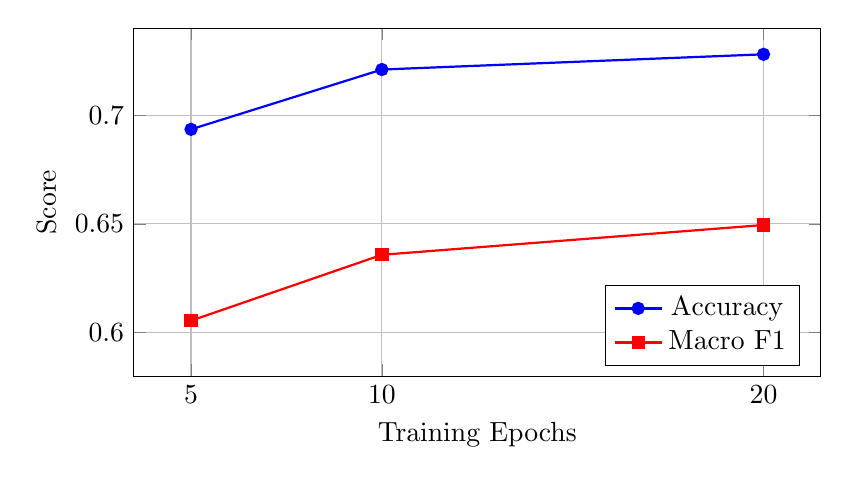
\begin{tikzpicture}
        \begin{axis}[
            width=0.85\textwidth,
            height=6cm,
            xlabel={Training Epochs},
            ylabel={Score},
            ymin=0.58,
            ymax=0.74,
            xtick={5,10,20},
            legend pos=south east,
            grid=major,
            ymajorgrids=true,
            xmajorgrids=true,
        ]
        \addplot[color=blue, mark=*, thick] coordinates {(5, 0.6935) (10, 0.7210) (20, 0.7280)};
        \addplot[color=red, mark=square*, thick] coordinates {(5, 0.6055) (10, 0.6358) (20, 0.6495)};
        \legend{Accuracy, Macro F1}
        \end{axis}
    \end{tikzpicture}
    \caption{Performance evolution of supervised ANN across training epochs.}
    \label{fig:supervised_evolution}
\end{figure}

\noindent In summary, training for additional epochs yields diminishing returns: the improvement from 5 to 10 epochs is moderate (+2.75 percentage points accuracy, +3.03 pp F1), while further training to 20 epochs provides only marginal gains (+0.70 pp accuracy, +1.37 pp F1).
This plateau suggests that the model's capacity to learn from the training data is approaching saturation.
Further improvements would likely require architectural changes, regularization techniques to address class imbalance, or data augmentation rather than extended training.
Also, the point of using this approach was showing how a lightweight head on top of embeddings can achieve good results with minimal training, which was accomplished.

\subsection{Zero-Shot Model Comparison}

The relationship between model size and zero-shot performance is non-trivial, as shown in Table~\ref{tab:zeroshot_size}.

\vspace{-15pt}
\begin{table}[htbp]
    \centering
    \caption{Zero-Shot Model Size vs Performance Trade-off}
    \label{tab:zeroshot_size}
    \begin{tabular}{lccc}
        \toprule
        \textbf{Model} & \textbf{Parameters} & \textbf{Accuracy} & \textbf{Macro F1} \\
        \midrule
        DeBERTa-v3-xsmall & 22M  & 0.6945 & 0.6226 \\
        BART-large-mnli   & 406M & 0.3765 & 0.3838 \\
        DeBERTa-v3-large  & 434M & \textbf{0.7170} & \textbf{0.6417} \\
        \bottomrule
    \end{tabular}
\end{table}

\noindent %The comparison reveals that model size is not directly correlated with performance.
The smallest model (DeBERTa-v3-xsmall, 22M parameters) dramatically outperforms BART-large (406M) by 31.8 percentage points in accuracy. %, demonstrating that \textit{training data composition matters more than parameter count}.
Looking at the training methodology for each model, the reason for this performance gap becomes clearer:

\begin{itemize}
    \item \textbf{DeBERTa-v3-xsmall}: Aggressively trained on human-labeled NLI datasets, including \textit{emotion classification tasks} in its training distribution. This direct exposure to emotion-related data provides strong inductive biases for this specific task.
    \item \textbf{DeBERTa-v3-large}: Trained on a mix of human-labeled and synthetic data, which increases diversity but sometimes makes it harder for the model to focus on the specific task. The additional 412M parameters provide only modest gains (+2.25 pp accuracy) over xsmall, suggesting diminishing returns when the training distribution already covers the target task.
    \item \textbf{BART-large}: Trained exclusively on MNLI without emotion data, resulting in poor transferability to emotion classification despite its large capacity.
\end{itemize}

\noindent The xsmall model's competitive performance (69.45\%, only 2.25 pp below the large variant) highlights an important practical insight: for emotion classification, a compact model trained on data relevant to the task at hand outperforms larger models trained on generic NLI corpora.
This suggests that, out of these three models in this specific context, DeBERTa-v3-xsmall offers the most optimal balance of performance and computational efficiency, particularly given that the task aligns with its training distribution. 
However, we can infer that if another task unrelated to the xsmall model's training data was to be solved, the large variant would likely outperform the small one due to its increased capacity and broader training data, making the performance difference more visible.

\subsection{Per-Class Performance Analysis}

Table~\ref{tab:per_class_comparison} compares per-class F1-scores between the best supervised model (ANN-20) and the best zero-shot model (DeBERTa-v3-large), revealing both approaches' strengths and weaknesses.

\vspace{-15pt}
\begin{table}[htbp]
    \centering
    \caption{Per-Class F1-Score Comparison: Supervised vs Zero-Shot}
    \label{tab:per_class_comparison}
    \begin{tabular}{lcccc}
        \toprule
        \textbf{Class} & \textbf{ Support } & \textbf{ ANN-20 } & \textbf{ DeBERTa-L } & \textbf{ $\Delta$ } \\
        \midrule
        Sadness  & 581 & 0.78 & 0.76 & +0.02 \\
        Joy      & 695 & 0.77 & 0.78 & -0.01 \\
        Anger    & 275 & 0.72 & 0.72 & 0.00 \\
        Fear     & 224 & 0.69 & 0.70 & -0.01 \\
        Love     & 159 & 0.52 & 0.48 & +0.04 \\
        Surprise & 66  & 0.42 & 0.41 & +0.01 \\
        \midrule
        \textbf{Macro Avg} & -- & \textbf{0.65} & 0.64 & +0.01 \\
        \bottomrule
    \end{tabular}
\end{table}

\noindent Both models perform best on high-frequency classes (sadness, joy: F1 $>$ 0.76) and struggle with rare emotions (surprise: F1 $\approx$ 0.41).
This may be caused by two diferent factors: the supervised model's limited exposure to rare classes during training, and the zero-shot model's reliance on general language patterns that may not capture the nuances of ambiguous emotions, especially those that are more complex.
The cap on the literature performance for this dataset (around 91\% according to Kermani et al. \cite{kermani2025systematicevaluationllmstrategies}) was achieved through fine-tuning, which enabled the model to learn the dataset's generator's distribution and idiosyncrasies, which is outside of this project's scope.

\subsection{Error Pattern Analysis}

\subsubsection{Supervised Learning Error Patterns}

Table~\ref{tab:supervised_confusions} presents the most frequent misclassifications for the best supervised model (ANN-20).
The \textbf{\%} column refers to the percentage of misclassified examples from the True class that were classified as the Prediction class.

\vspace{-15pt}
\begin{table}[htbp]
    \centering
    \caption{Top 5 Confusion Patterns: Supervised ANN (20 epochs)}
    \label{tab:supervised_confusions}
    \begin{tabular}{llcc}
        \toprule
        \textbf{True} & \textbf{Prediction} & \textbf{Count} & \textbf{\%} \\
        \midrule
        Love     & Joy     & 61 & 38.4\% \\
        Sadness  & Joy     & 74 & 12.7\% \\
        Anger    & Joy     & 31 & 11.3\% \\
        Surprise & Joy     & 19 & 28.8\% \\
        Surprise & Fear    & 15 & 22.7\% \\
        \bottomrule
    \end{tabular}
\end{table}

\noindent The dominant error pattern is over-prediction of ``joy'', the most frequent class (33.5\% of training data).
This suggests the model has learned a bias toward the majority class, a relation that appears to be further amplified for emotions that are related to joy, as these examples become easier to confuse between.
For example, the text \textit{i got home feeling hot tired and great} was labeled as ``love'' instead of ``joy'' which is not necessarily wrong, but rather ambiguous. 

\noindent The confusion between the ``sad'' and ``joy'' labels may seem counterintuitive, but, upon closer inspection, we find examples such as \textit{i stop feeling guilty}, an example labeled as ``sad'' but that could be interpreted as ``joy'' as well depending on context.
Additionally, as mentioned previously, the dataset itself has many ambiguous or poor classifications, which could also cause these types of misclassifications.

\subsubsection{Zero-Shot Error Patterns: DeBERTa Models}

In contrast to BART, DeBERTa models exhibit balanced error distributions similar to supervised approaches, as shown in Table~\ref{tab:deberta_confusions}.

\begin{table}[htbp]
    \centering
    \caption{Top 5 Confusion Patterns: DeBERTa-v3-large}
    \label{tab:deberta_confusions}
    \begin{tabular}{llcc}
        \toprule
        \textbf{True Label} & \textbf{Predicted As} & \textbf{Count} & \textbf{\% of Class} \\
        \midrule
        Love     & Joy     & 48 & 30.2\% \\
        Love     & Sadness & 22 & 13.8\% \\
        Surprise & Joy     & 14 & 21.2\% \\
        Surprise & Sadness & 9  & 13.6\% \\
        Fear     & Sadness & 22 & 9.8\% \\
        \bottomrule
    \end{tabular}
\end{table}

\noindent DeBERTa's errors mirror those of the supervised model (love $\rightarrow$ joy, surprise $\rightarrow$ joy/fear/sadness), indicating these confusions reflect genuine semantic ambiguity rather than issues with the model itself, as proven by 
the examples on the supervised learning section.
The convergence of error patterns between supervised and zero-shot approaches suggests both are capturing similar linguistic regularities in the data.

\noindent Notably, the small DeBERTa variant (xsmall) exhibits similar confusion patterns to its larger counterpart, further supporting the conclusion that \textit{training data composition dominates over parameter count}\cite{app11020796}.
The xsmall model's inclusion of emotion classification tasks in its training distribution (among 33 NLI datasets labeled by humans) likely explains its strong performance despite limited capacity, while the large variant's mixed training approach provides only marginal improvements for this specific task (although generalization to other tasks benefits from the increased capacity and data diversity).

\subsubsection{Zero-Shot Error Patterns: BART Failure Case}

BART-large-mnli's catastrophic failure (37.65\% accuracy) is explained by extreme prediction bias toward ``surprise'', as shown in Table~\ref{tab:bart_confusions}.

\vspace{-15pt}
\begin{table}[htbp]
    \centering
    \caption{Top 5 Confusion Patterns: BART-large-mnli}
    \label{tab:bart_confusions}
    \begin{tabular}{llcc}
        \toprule
        \textbf{True Label} & \textbf{Predicted As} & \textbf{Count} & \textbf{\% of Class} \\
        \midrule
        Joy      & Surprise & 362 & 52.1\% \\
        Love     & Surprise & 79  & 49.7\% \\
        Fear     & Surprise & 110 & 49.1\% \\
        Sadness  & Surprise & 266 & 45.8\% \\
        Anger    & Surprise & 125 & 45.5\% \\
        \bottomrule
    \end{tabular}
\end{table}

\noindent BART predicts ``surprise'' for approximately 50\% of \textit{all} classes, resulting in:
\begin{itemize}
    \item 86\% recall for surprise (57/66 correct predictions)
    \item Only 6\% precision (57 correct out of 999 total ``surprise'' predictions)
\end{itemize}

\noindent This failure likely stems from the hypothesis template used in zero-shot classification: \textit{``This text expresses surprise''}.
BART's pre-training on MNLI may have caused it to assign disproportionately high entailment scores to this specific phrasing, regardless of actual text content.
This highlights a critical limitation: zero-shot performance is highly sensitive to hypothesis template design and biases created during pre-training.

\newpage

\section{Conclusion}
This project explored natural language classification using both supervised learning (artificial neural networks) and zero-shot approaches (pre-trained transformer models). 
Our experiments show that the 20-epoch supervised model achieved the most competitive performance (though increasing training epochs had clear diminishing returns), while zero-shot models, especially those trained on relevant data, can closely match supervised results.

\noindent Additionally, the compact DeBERTa-v3-xsmall zero-shot model, trained on emotion datasets, outperformed a much larger model, BART-large-mnli, which lacked such targeted data, and performed similarly to DeBERTa-v3-large, a much larger model trained on similar data. 
These results backed the conclusion that, while increasing model size can provide marginal gains, the relevance and composition of training data are often more decisive for specialized tasks. 

\noindent Analyzing the dataset, we also observed that class imbalance and label ambiguity in the dataset present significant challenges for classification models, effectively capping performance if no fine-tuning technique is used.
These issues translated into both model types making similar misclassifications, which were many times more connected to actual ambiguous labels instead of an inability to generically perform the task.

\noindent Overall, our results suggest that both supervised and zero-shot approaches are viable for emotion classification, with model selection and training data relevance, and dataset quality playing major roles in determining success. 

\paragraph{Note:} Generative AI was used moderately across the development of this project to help with minor tasks in code and writing.
This use was done with extreme caution, as every decision ultimately fell back onto us, the authors, and each generation and completion was carefully analyzed as if it were our own.
We aimed to strike a balance that would allow us use AI's strengths to save time in this process without ever compromising the project's scientific quality.

\bibliography{references}

\end{document}